\section{Antennentheorie}
\subsection{ Was ist eine Antenne}
Bevor in die Antennentheorie und das Abstrahlverhalten von Antennen betrachten, soll zuerst geklärt werden, was eine Antenne ist. Und wie sieht das Grundprinzip aus, welches das Abstrahlen einer elektrischen Welle die in einem Leiter geführt wird, in ein elektromagnetisches Wechselfeld übergeht und abgestrahlt wird. \\
Was ist eine Antenne:
\begin{itemize}
\item alle oszillierenden elektrischen und magnetischen Felder strahlen
\item alle Leitungen die einen Wechselstrom führen strahlen
\item Antennen ermöglichen das kontrollierte abstrahlen von elektrischer Energie in den Freienraum und wider zurück in die Leitung

\end{itemize}

\begin{tabular}{l}
\hline 
Antennen Design Faktoren \\ 
\hline 
Die in verschiedene Richtungen abgestrhalte Energie wird (antenna pattern) genannt\\ 
\hline 
Die total abgestrahlte Leitung verglichen mit der zugeführten Leitung ist die Abstrahleffizienz \\ 
\hline 
Anpassung ist der Vergleich der  Antennen Impedanz  und der Impedanz der Transmission Line\\ 
\hline 
Die Abstrahlung ist eine Funktion der Frequenz \\ 
\hline 
• \\ 
\hline 
\end{tabular} 

Die Grundlge jeglicher abstrahlung von elektromagenischen Feldern ist der Wechselstrom. Aus der Wechselstromlehre ist bekannt, dass ein sich ändernendes Elektrishes Feld in einem Leiter ein en sich änderenden Strom hervorruft. und jeder Strom ein Magnetfeld mitsich bringt. Witer jede s sich änderne Magnet Ferld bewirkt eien Änderung des Elektrischen Feldes. Daraus wird klar, dass ein Elektrischesfeld ein Magnetfeld  hervorruft und umgekehrt. Oder das eine kann ohne das andere nicht existeiren. Ein Wechsel des Elektrischenfeld führt zu einer Änderung des Magneischenffeld. Das gilt in einer Leitung aber auch im freien Raum.

Die Maxwell Gelichungen zeigen diesen Zusammenhang mathematisch auf.
\[\bigtriangledown x H =\frac{dD}{t}\]
\[\bigtriangledown x E =\frac{dB}{t}\]

Die Geschwindigkeit mit der sich eine Elektromagnetische Welle im freien Raum oder in eriner Leitung ausbreitet ist von den Materialeigenschaften des Mediums abhänig.\\
Im Vakuum gilt:
\[v_{p} =\frac{1}{\sqrt{\mu\varepsilon}}\]

\subsection*{offene Leitungs als Stralher}
Um zu erkennen, dass eine Antenne in ihrer simplen form als Strahlendes Elementwirkt, muss zuerst die Leitungstheorie verstanden sein.
Wir gehen von einer Spannugnsquelle VG mit einer Quelleimpedanz ZG aus. Diese Quelle wird eine Leitung mit einem Abschlusswiderastand ZL verbunden. Die Quelle führt zu einer Spannungswelle in der Leitung. Die Spannungswelle ist in eine vor und in eine rücklaufende Welle geteilt. Über das Ohmsche Gesetzt ist der Strom in der Leitung definiert. Genauso wie die Spannungswelle einen Vor und einen Rückanteil besitzt, besitzt auch die Stromwelle eine vor- und rücklaufende Welle.
\[V(z) = V0*e^{-\beta*z}+V0*e^{\beta*z}\]
und
\[I(z) = \dfrac{V0}{Z0}*e^{-\beta*z}-\dfrac{V0}{Z0}*e^{\beta*z}\]

Die Wechselspannungsquelle treibt die Transmision Line mit der Impedanz Z0.

Eine hypothetische verlustlose Antenne, die gleichmässig in alle Raumrichtungen abstrahlt beziehungsweise aus allen Richtungen empfängt, wird isotroper Strahler oder Kugelstrahler genannt. Als Sendeantenne erzeugt sie eine Kugelwelle mit sphärischen Phasenfronten. Im Abstand r gilt winkelunabhängig folgende Leistungsdicht:
% \[S=\frac{P_{S}{4r}\]
\[S=\frac{P_{S}}{4 \pi r^{2}}\]
wobei $P_{S}$ die gesamt abgestrahlte Wirkleistung bezeichnet.


\subsection{ Antennen als Wellenwandler}
Antennen erzeugen und empfangen elektromagnetische Wellen, die sich im freien ausbreiten. Im Sendefall wandelt die Antenne, die ihr zugeführte Leitung möglichst effizient in elektromagnetische Wechselfelder um. Im Empfangsfall nimmt die Antenne aus einem elektromagnetischen Wellenfeld Leistung auf und stellt sie an einem Netzwerktor zur Verfügung. \\
Eine Signalübertragung mit zwei Antennen ist im folgenden Bild gezeigt. Eine leitergeführte Welle wird an ein Eingangstor (das Tor 1) geführt. Das Tor 1 stellt den Fusspunkt und somit der Anschlusspunkt einer Antenne dar. Die leitergeführte Welle wird am Tor 1 idealerweise reflexionsfrei aufgenommen. Die Antenne erzeugt ein Wechselfeld. Dabei agiert als Wandler der leitergeführten Welle in eine Freiraumwelle. Die Freiraumwelle führt Leitung von der Antenne fort. Mit wachsendem Abstand erscheinen die Wellen als Ebenen. Dabei spricht man vom Fernfeld. Antennen besitzen eine Dualität, das bedeutet ein Element welches gute abstrahlende Eigenschaften aufweisst, besitzt ebenso gute Eigenschaften als Empfänger für elektromagnetische Wellen. \\
Im Empfangsfall nimmt eine Antenne Energie aus dem Wellenfeld auf und regt eine Leitergebundene Welle an ihrem Netzwerktor (Tor 2) an.
\subsection{Nahfeld und Fernfeld}
Bei der Beschreibung der elektromagnetischen Wellenfelder um eine Antenne, ist die Distanz zur Antenne von grosser Bedeutung. Es macht einen grossen Unterschied ob man die Feldverteilung in der unmittelbaren Umfeld der Antenne ( dem Nahfeld) oder den Beobachtungspunkt in einer grossen Entfernung (dem Fernfeld) ansetzt.
Im Fernfeld steht das Elektrische E Feld  und das Magnetische H Feld senkrecht  im 90$^\circ$Winkel aufeinander. Die Wellenfront der beiden Felder bewegt sich in Ausbreitungsrichtung wie eine senkrechte Ebene vorwärts.\\
Die Feldverteilung des elektromagnetischen Wechselfeld kennt drei markante Zonen:
\begin{itemize}
\item Reaktives Nahfeld
\item Strahllendes Nahfeld 
\item Fernfeld
\end{itemize}
 Der Übergang vom Nahfeld zum Fernfeld einer Antenne ist fliessend und es können keine klaren Abgrenzungen gezogen werden. Das Nahfeld zeichnet sich ander als das Fernfeld durch seine star reaktiven Feldanteile aus. Im reaktiven Nahfeld wird pendelt elektrische und magnetische Energie zwischen der Antenne und dem Freiraum hin und her. Diese Energie wird rund um die Antenne gespeichert.
Im Fernfeld dominiert radial orientierte Leistungstransport. 
\\Historisch gesehen haben sich bei der  analytischen Betrachtung von Strahlungsproblemen unterschiedliche Näherungen (Fresnel Näherung und die Fruenhofer Näherung) bewährt. Hieraus haben sich Formeld für den Abstand den man zur Antenne einnehmen muss, wenn man mit den für das Fernfeld definierten Antennenkenngrössen arbeiten wil. Daraus ergibt sich den Ferfeldabstand. Der Fernfeldabstand hängst von der verwendeten Wellenlängen $\lambda$ und den geometrischen Abmessungen der Antenne ab. Die Näherung für das Fernfeld für elektrisch kurze Antenne tretten ab mindestens einem Abstand von r0 ein.
\[r0=2*\lambda\]
Bei Antennen deren grösste Antennenabmessungen grösser als die Wellenlänge $\lambda$ sind, treten die Fernfeldbedingungen erst bei grösseren Abständen ein.
\[r0=\dfrac{2D^2}{\lambda}\]
Mit:\\d0: Minimale Distanz für die Annahme des Fernfeld Kriterium\\
D: Grösstes des Anten mass in Meter\\
$\lambda$: Wellenlänge
\todo{quelle vom bild einfügen}
%https://de.wikipedia.org/wiki/Nahfeld_und_Fernfeld_%28Antennen%29
\begin{figure}[htbp]
	\centering
		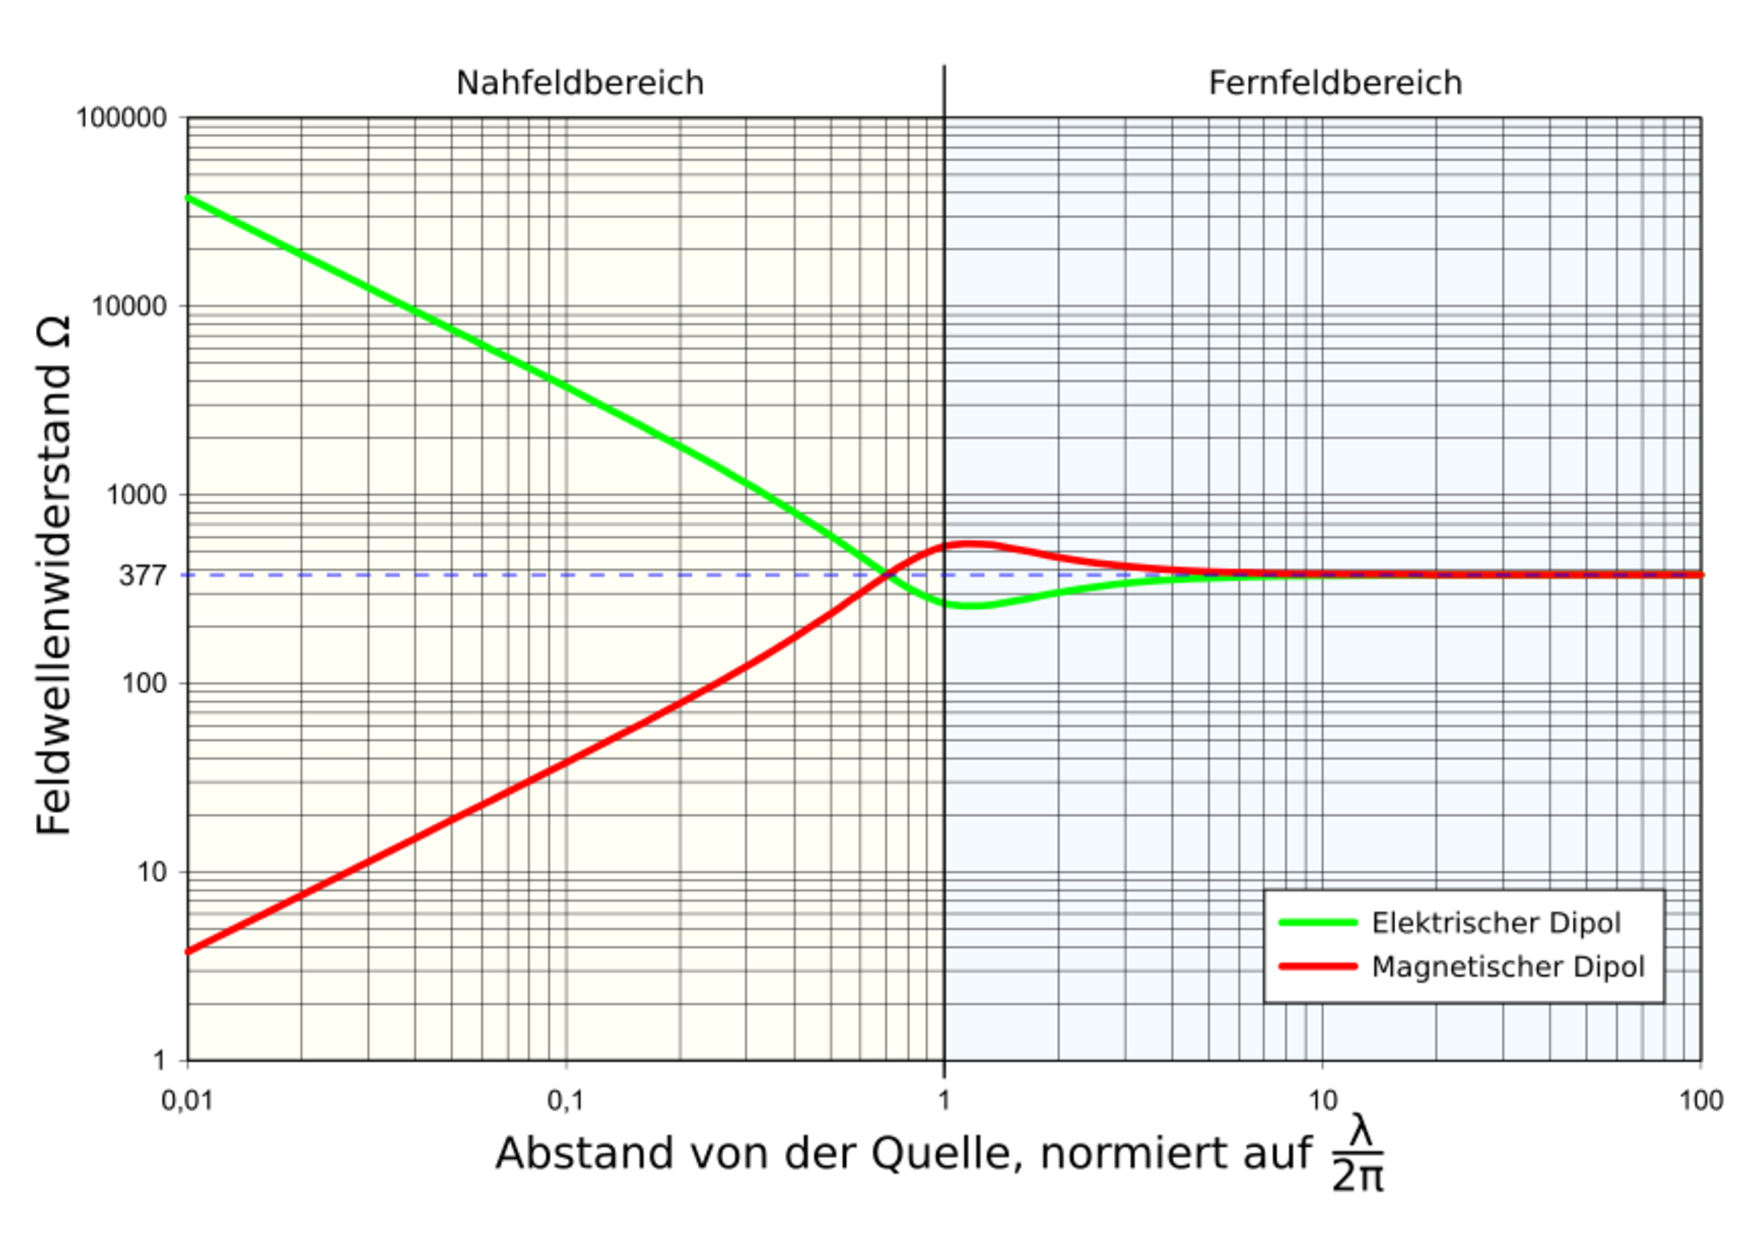
\includegraphics[width=6cm]{content/bilder/Feldwellenwiderstandsverlauf_im_Nahfeld-Fernfeld.pdf}
	\caption{Nah-Fernfeld}%
	\label{Nah-Fernfeld}
\end{figure}
Das Fernfeld $(r \rightarrow \infty$ einer Antenne hat volgende Eigenschaften:

\begin{itemize}
\item Die beiträge der Feldgrössen E und H sind reziprok zum Abstand r betrag E ,Betrag H tilde 1/r
\item Die Amplituden der Feldgrössen E und H sind in Phase
\item Der Feldwellenwiderstand $Z_{F0}$ verknüpft die Feldgrössen: $ E=Z_{F0}*H$
\item Die Wellenfront der elektromagnetischen Wellen erscheinen als ebene Wellen
\item Die Vektoren der Transversalen Welle besitzen nur noch transversale Anteile
\item ...
\item ...
\end{itemize}
\subsection{Kenngrössen von Antennen}
Die wichtigsten elektromagnetischen Eigenschaften von Antennen für den Einsatz in Funktsystemen lassen sich durch eine Reihe von Kenngrössen beschreiben. Um diese Kenngrössen und ihre Berechnung besser zu veranschaulichen werden sie anhand des Hertzschen Dipol angewendet. Der Hertzsche Dipol ist im Kapitel xxx beschrieben. 
\subsubsection{Richtdiagramm}

Im Fernfeld nimmt die Krümmung der sphärischen Phasenfront einer Kugel immer ab. Für r gegen unendlich kann die Kugelwelle lokal durch eine homogene ebene Welle angenähert werden. Die transversalen Feldkomponenten werden phasengleich ind es wird nur in radialer Richtung Wirkleistung transportiert. Der Richtwirkung im Raum wird kommt eine grosse praktische  Bedeutung zu. Von ihr hängt es ab, welcher Anteil der gesamten ausgestrahlten Leitung effektiv für den eigentlichen Verwendungszweck genutzt wird. Je nach Verwendungszweck des Antennensystem ist eine bestimmt Feldverteilung über den Raum verlangt. Die Verteilung der Strahlung in verschieden Raumrichtungen liefert die Verteilung der Feldstärke in Abhängigkeit des Raumwinkels einer Antenne. Der Raum winkel wird in Kugelkoordinaten mit den Angaben über theta und phi gemacht. Eine Aussage über die Richtcharakteristik wird oft im Fernfeld gemacht.

Die Richtcharakteristik eines hypothetischen Kugelstrahlers ist 1, das heisst die abgestrahlte Leitung ist unabhängig von theta oder phi. Die Richtcharakteristik eines in Z ausgerichteten Hertzschen Dipols ist $sin(\theta) $ in polarkoordinaten ist ein doppel Kreis sichtbar. Die maximale Richtwirkung des E Feld lieg in der xz Ebene bei einem theta Winkel von 90 $^\circ$. Das ist naheliegend, denn bei$\frac{\lambda} {2} $ ist der sinus 1.


Anstelle von aufwendigen dreidimensionalen Richtdiagrammen kommen zweidimensionale Schnitte durch den Antennenmittelpunkt als Phsenzentrum und dem Maximum der Feldverteilung zum einsatz. Oft geben das vertikale Richtiagramm mit theat und phi und das horizontale Richtdiagramm mit theat = $\frac{\lambda} {2} $ und phi angegeben.

Ein Mass für den Grad der Energiebündelung bei Richtantennen ist die Breite der Strahlungskeule. Sie wirdausgedrückt durch die vertikalen und horizontalen Halbertsbreiten delta $\theta$ und delta $\phi$ der Hauptkeulen.Das ist der Winkelbereich, innerhalb dessen die Strahlungsdichte um nicht mehr als die Hälfte der maximalen Strahlungsdichte absinkt. Das bedeutet, die Strahlugsdichte sink um 3dB ab. Die Feldstärke fällt in diesem Bereich höchstens um $\frac{1} {sqrt(2)} =70.7 Prozent $ ihres Maximalwertes ab.

Beim Hertzschen Dipol entnimmt man dem vertikalen Richtiagramm in der zx Ebene einen Öffnungswinkel von  90 $^\circ$ 

\subsubsection{Richtfaktor und Gewinn}










\subsection{elementarer Antennen Dipole}
\subsubsection{Hertzscher Dipol}
Ein elektrisch kurzer Linearstrahler der länge $l<<\frac{\lambda_{0}}{4}$ kann als konzentriertes Bauelement betrachte werden. Auf seiner gesamten Länge kann die komplexe Amplitude $\underline{I}$ eine räumlich konstante Stromverteilung, die zeitlich sinusförmig schwingt, annehmen.
\subsubsection{Fitzgeraldscher Dipol}
\subsection{Antennenbauformen}
\subsection{symmetrisch gespiesene Antennen}

Es gibt zwei Grundantennenformen, den Hertzschen Dipol und den Fitzgeradscher Dipol. Beide sind symmetrisch gespiesene Antennen. Im Nahfeld des Hertschen Dipols überwiegt das E Feld also der kapazitive Anteil, während im Nahfeld des Fitzgeradschen Dipols das H Feld also der induktive Anteil überwiegt. Im Fernfeld sind bei beiden Antennen das H und E Feld gleich stark und nehmen mit zunehmendem Abstand $1/r$ab. \\
Die Ausrichtung des E und H Feld sind bei den beiden Antennen verschieden. \\
Das E Feld eines Hertschen Dipols ist im Fernfeld gleich polarisiert wie der Dipol. \\
Genau umgekehrt ist das Feld des Fitzgeralschen Dipols. Das H Feld ist in der selben Ebene wie der Dipol. 

\begin{itemize}
\item Bauform
\item el. mag Feld Ausrichtung
\item Impedanz der $\lambda /2 $ Antenne
\item Beschreibung des Feld
\item el. mag Feld Ausrichtung
\item Impedanz der $\lambda /2 $ Antenne
\item Richtcharakteristik
\end{itemize}
\subsubsection{$\lambda /2 $ Dipol Antenne}
Die $\lambda /2 $ Dipol Antenne ist eine der am Meisten eingesetzten Antennen. In diesem Abschnitt wird die Dipolantenne mit einer sehr dünnen Radius  deren Länge einer halben Wellenlänge entspricht betrachtet. 

Eine Dipol Antenne mit der Länge L entlang der Z-Achse orientiert ist und z = 0 ist, fliesst der Strom in der z-Richtung mit einer Amplitude, die der folgende Funktion entspricht:
$I(z)=\begin{cases}I_{0}sin[k(\frac{L}{2}-z)],& 0\le z \le \dfrac{L}{2} \\ I_{0}sin[k(\frac{L}{2}+z)], & -\dfrac{L}{2} \le z \le 0 \end{cases}$

%\begin{tikzpicture}[xscale=0.04,yscale=0.08,domain=0.125:220,samples=400]
%    \draw[->] (-10,0) -- (225,0) node[below] {$x$};
%    \draw[->] (0,-5) -- (0,45) node[left] {$y$};
%    \foreach \i in {50,100,...,200} {
%        \draw (\i,1) -- (\i,-1) node[below] {$\i$};
%    }
%    \foreach \i in {10,20,...,40} {
%        \draw (1,\i) -- (-1,\i) node[left] {$\i$};
%    }
%    \draw[blue] plot (\x,{40-0.2*\x});
%    \draw[red] plot (\x,{5/\x});
%\end{tikzpicture}

Bei einem Dipol mit der Länge  $L= \frac{\lambda}{2}$ sich einen Strombauch über dem Einspeise Punkt ausbildet und der Strom zu den Enden gegen null geht.\\
Ein Dipol mit der Länge  $L= \lambda$ bilden sich zwei  Strombauche über die ganze Länge des Dipols aus. Beim Einspeise Punkt und den beiden Enden geht der Strom gegen null.\\
Wichtig bei der Stromverteilung ist, dass der Strom  in der Zeit sinusförmig  mit der Frequenz f oszilliert. 


%Abbildung \nodepart{•}; Stromverteilungen auf endlich langen Dipol-Antennen.

Die Eingangsimpedanz eines Dipols ist Abhängigkeit von seiner Länge. Man beachte, dass die Eingangsimpedanz wird als Z = R + jX, wobei R der Widerstand und die Reaktanz X angegeben. Die Reaktanz X ist steht für die im Nahfeld gespeicherte Feldenergie.

%Abbildung 2. Eingangsimpedanz in Abhängigkeit von der Länge (L) einer Dipolantenne.

Man beachte, dass für sehr kleine Dipolantennen, ist die Eingangsimpedanz kapazitiv ist, das heisst, die Impedanz durch eine negative Reaktanz-Wert (und eine relativ kleine reale Impedanz oder Widerstand) dominiert. Wir der Dipol länger, so erhöht sich der Eingangswiderstand, zusammen mit der Reaktanz. Bei etwas weniger als $L=\frac{\lambda}{2}$ hat die Antenne Nulldurchgang des Imaginärteils.

Wenn die Länge des Dipol-Antenne ist nahe der Wellenlänge ist, wird die Eingangsimpedanz unendlich. Als einfachere Erklärung, kann der Stromverteilung einer $L = \lambda$ langen Antenne betrachtet werden. ES ist ersichtlich, dass bei der Einspeisestelle der Strom gegen Null geht. Unter Berücksichtigung, dass der Strom nach dem Ohmschen Gesetz $I = \frac{U}{R}$ ist, so ist naheliegen, dass der Widerstand gegen unendlich gehen muss. 

Im nächsten Abschnitt werden wir das Strahlungsmuster Dipol-Antennen zu berücksichtigen.


Strahlungsdiagramme für die Dipol-Antennen

Die weit Felder aus einer Dipolantenne der Länge L sind gegeben durch:
\[E_{\theta}=\frac{j\eta I_{0} e^{-jkr}}{2\pi r}\frac{cos(\frac{kL}{2}cos(\theta))-cos(\frac{kL}{2}))}{sin(\theta)}\]

\[H_{\Phi}=\frac{E_{\Theta}}{\eta}\]

Die normierten Strahlungsmuster für Dipolantennen verschiedener Längen sind in Abbildung 3 dargestellt.


Abbildung 3. normalisierte Strahlungsmuster für die Dipol-Antennen der angegebenen Länge.

Die Full-Wellenlängen-Dipol-Antenne ist richtungs als die kürzere Viertelwellenlängen-Dipol-Antenne. Dies ist ein typisches Ergebnis der Antennentheorie: es dauert eine größere Antenne allgemein Richt erhöhen. , Die Ergebnisse sind jedoch nicht immer offensichtlich. Das 1,5-Wellenlängen-Dipol-Muster ist ebenfalls in Figur 3. Anmerkung aufgetragen dass dieses Muster ein Maximum bei etwa +45 und -45 Grad.

Die Dipolantenne ist symmetrisch, wenn azimutal angesehen (um die lange Achse des Dipols); als Ergebnis das Strahlungsmuster nicht eine Funktion des Azimutwinkels. Damit ist die Dipolantenne ein Beispiel einer Rundstrahlantenne. Ferner hat das E-Feld nur eine Vektorkomponente und damit die Felder linear polarisiert. Wenn sie in der XY-Ebene betrachtet wird (für einen Dipol entlang der z-Achse orientiert ist), wird die E-Feld in der -y-Richtung, und folglich wird die Dipolantenne ist vertikal polarisiert.

Das 3D-Motiv für das 1-Wellenlängen-Dipol-Antenne ist in 4 gezeigt Dieses Muster ist ähnlich dem Muster für die Viertel- und Halbwellen-Dipolantenne.


Abbildung 4. Normalized 3d Strahlungsmuster für die 1-Wellenlängen-Dipol-Antenne.

Die 3D-Strahlungsmuster für die 1.5-Wellenlängen-Dipol-Antenne unterscheidet sich signifikant und wird in 5 gezeigt.


Abbildung 5. Normalized 3d Strahlungsmuster für die 1,5-Wellenlängen-Dipol-Antenne.
Das (peak) Richtcharakteristik der Dipolantenne variiert, wie in Figur 6 gezeigt.


Abbildung 6. Dipole Antenna Richtwirkung als eine Funktion der Dipollänge.

Abbildung 6 zeigt, dass bis zu etwa L = 1,25 Die Richt steigt mit der Länge. , Für größere Längen die Richtwirkung hat jedoch einen Aufwärtstrend ist aber nicht mehr monoton.

Im nächsten Abschnitt werden wir am häufigsten Dipol-Antenne, die Halbwellen-Dipol-Antenne suchen.
\begin{itemize}
\item Fusspunkt Impedanz
\item Feldausbreitung im Nahfeld
\item Feldausbreitung im Fernfeld
\item Im Nahfeld relevant
\item Richtcharakteristik
\end{itemize}
\subsubsection{Loop Antenne}
Die Loop Antenne ist eine symmetrisch gespiesene Antenne. eine Loop Antenne ist einem Fitzgeralschen Dipol nach empfunden. Die Loop Antenne wird durch eine dünne Leiterschleife mit einem Radius  $r=\dfrac{bla}{bla}$  dargestellt. \\
Im Nahfeld der Loop Antenne dominiert der xx Anteil. Das E Felde ist in der Ebene der Leiterschleife. Das H Feld erscheint 90$^\circ$Winkel zum E Feld. 
\subsection{Abstrahlcharakteristik}
\subsubsection{Monopol über leitendem Ground}
In der Praxis werden Monopolantennen über Masseflächen mit endlicher Leitfähigkeit und endlicher Grösse verwendet. Dies beeinflusst die Eigenschaften der Monopolantennen, insbesondere das  Strahlungsmuster. Die Impedanz der Monopolantenne wird minimal über einem endlichen grossen Massebene verändert. Voraussetzung hierfür ist, dass die Massebene  im Durchmesser über einige  Wellenlängen der Abstrahlfrequenz besitzt. Jedoch ist die Strahlungscharakteristik der Monopolantenne stark durch eine endliche Grösse Massebene beeinflusst. Das resultierende
 Strahlungsdiagramm strahlt in einer "schrägen" Richtung, weg von
  der horizontalen Ebene. Ein Beispiel für das Strahlungsmuster für eine 
  $\dfrac{\lambda}{4}$ 
  Monopolantenne mit einem Durchmesser der Massenfläche von 3 Wellenlängen. 
  Die  $\dfrac{\lambda}{4}$  Monopolantenn ist in der positiven z Richtung ausgerichtet.

%Strahlungsmuster der Monopolantenne aufgrund der endlichen Grösse Massebene.

Das resultierende Strahlungsmuster für diese Monopolantenne ist  omnidirektionalen. Jedoch hat die Richtung der maximalen Strahlung von der xy-Ebene in einem Winkel von dieser Ebene angehoben verändert. Im Allgemeinen gilt je  grösser Grundplatte ist, desto niedriger ist diese Richtung der maximalen Strahlung. Das bedeutet wenn die Grundebene sich gegen  unendlich nähert, so liegt die maximale  Strahlung  in der xy-Ebene.
%\cite{http://www.antenna-theory.com/antennas/monopole.php}

Der Antennengewinn ist  um 3 dB besser als eine Dipol Antenne. Da die Monopolantenne ihr Feld nur über dem perfekt leitendem Untergrund aufbaut.
